% Created 2019-05-16 jue 21:30
% Intended LaTeX compiler: pdflatex
\documentclass[11pt]{article}
\usepackage[utf8]{inputenc}
\usepackage[T1]{fontenc}
\usepackage{graphicx}
\usepackage{grffile}
\usepackage{longtable}
\usepackage{wrapfig}
\usepackage{rotating}
\usepackage[normalem]{ulem}
\usepackage{amsmath}
\usepackage{textcomp}
\usepackage{amssymb}
\usepackage{capt-of}
\usepackage{hyperref}
\author{Marco Centurion}
\date{\today}
\title{Manual de Instalación}
\hypersetup{
 pdfauthor={Marco Centurion},
 pdftitle={Manual de Instalación},
 pdfkeywords={},
 pdfsubject={},
 pdfcreator={Emacs 26.1 (Org mode 9.1.9)}, 
 pdflang={English}}
\begin{document}

\maketitle
\tableofcontents

\section{Descripción}
\label{sec:org5c161cf}
El presente documento describe los pasos para instalar el software
desarrollado en el marco del proyecto de grado "Ingeniería Dirigida
por Modelos aplicada a la configuración de redes de computadoras".
\section{Dependencias}
\label{sec:org4b39ff3}
Para instalar el software es necesario contar con una instalación
existente del Entorno de Desarrollo \texttt{Eclipse}, con algunos paquetes
extra.
\subsection{Resumen}
\label{sec:org2f21645}

De forma resumida, se precisa el siguiente ambiente configurado:

\begin{itemize}
\item \texttt{Eclipse Modeling Tools} \footnote{\href{https://www.eclipse.org/downloads/packages/release/2008-09/r/eclipse-modeling-tools}{Página de descarga de Eclipse Modeling Tools}} 2018-09
\item \texttt{Papyrus} \footnote{\href{https://www.eclipse.org/papyrus/}{Página principal del proyecto Papyrus}} 4.1.0.201809120950
\item \texttt{Acceleo} \footnote{\href{https://www.eclipse.org/acceleo/}{Página principal del proyecto Acceleo}} 3.7.8.201902261618
\end{itemize}

Las versiones referenciadas son últimas con las que se testeó el
software, sin perjuicio de que el mismo funcione correctamente con
versiones más nuevas.
\subsection{Eclipse}
\label{sec:org721ce9f}

Para la instalación de \texttt{Eclipse} se recomienda utilizar la herramienta
\texttt{Eclipse Oomph}\footnote{\href{https://projects.eclipse.org/projects/tools.oomph}{Página principal de Eclipse Oomph}}. Luego de descargar \texttt{Oomph}, se debe ejecutar,
lo que presenta la siguiente ventana, en la cual se selecciona
\texttt{Eclipse Modeling Tools}:

\begin{center}
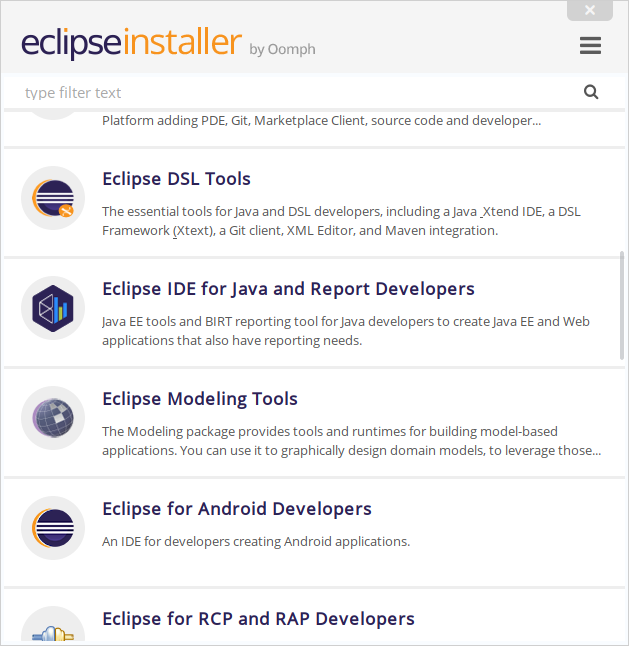
\includegraphics[width=.9\linewidth]{images/oomph_main.png}
\end{center}

En la siguiente ventana se debe seleccionar la versión \texttt{2018-09}:

\begin{center}
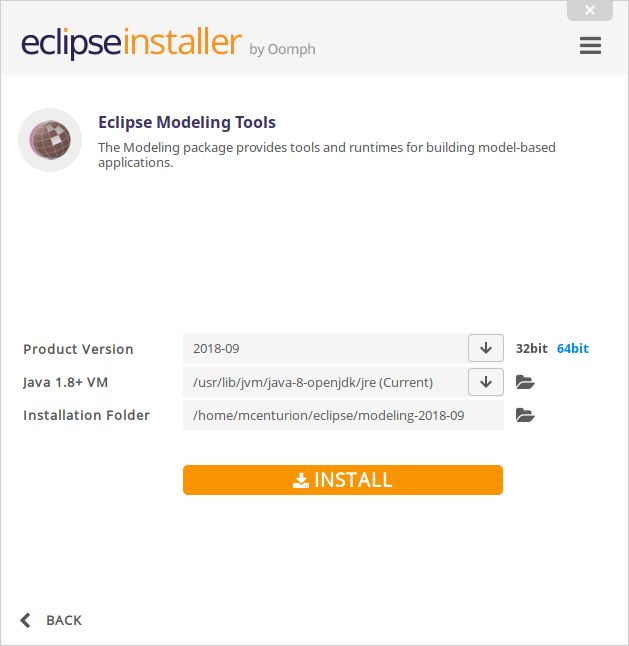
\includegraphics[width=.9\linewidth]{images/oomph_selection.png}
\end{center}

Al hacer click en \texttt{Install} comienza la instalación, durante la cual
se presentan varias licencias que se deben aceptar para continuar con
la instalación.

Luego de completada la instalación, \texttt{Oomph} permitirá ejecutar \texttt{Eclipse}:

\begin{center}
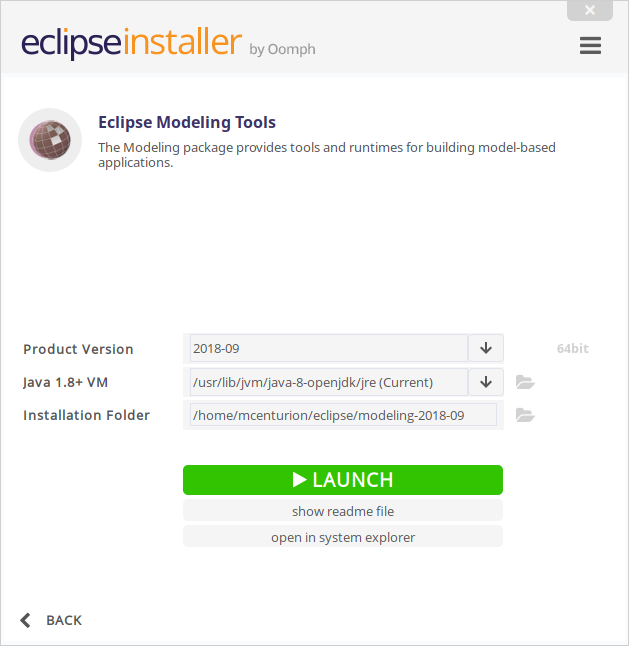
\includegraphics[width=.9\linewidth]{images/oomph_launch.png}
\end{center}

Esto completa la instalación de \texttt{Eclipse}

\subsection{Paquetes}
\label{sec:org82d9ff1}

Todos los paquetes a instalar se encuentran en los repositorios por
defecto de eclipse.
\subsubsection{Papyrus}
\label{sec:orgedb7b37}
\texttt{Papyrus} se instala desde el diálogo de instalación de software de
\texttt{Eclipse}, que se encuentra en "Help > Install New Software\ldots{}".

Al seleccionar como fuente "--All Available Sites--" , se puede
encontrar \texttt{Papyrus for UML} bajo la categoría "Modeling":

\begin{center}
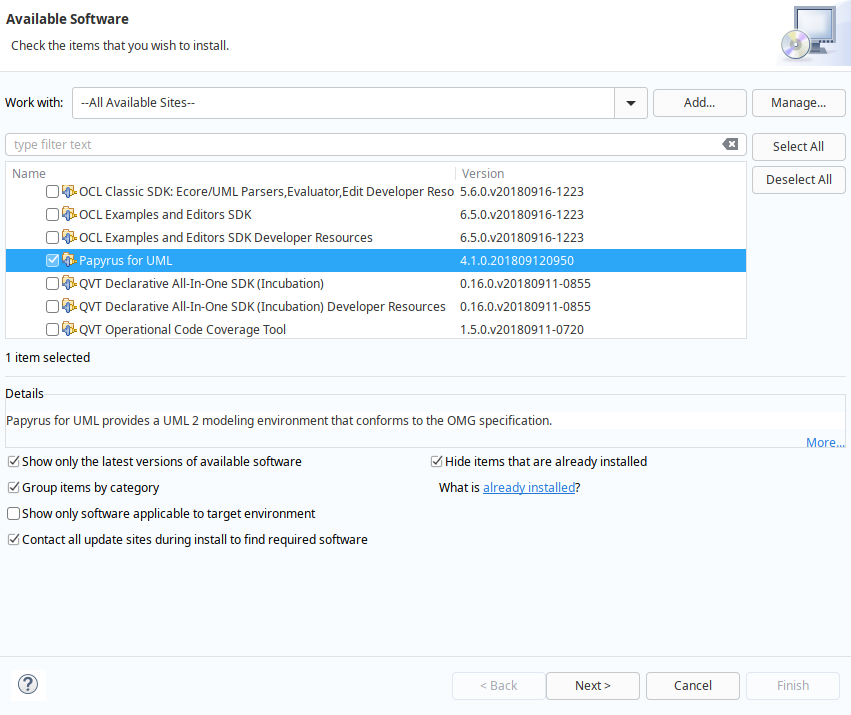
\includegraphics[width=.9\linewidth]{images/papyrus.png}
\end{center}

Luego de seleccionada la opción, se debe continuar con el proceso de
instalación, aceptando las licencias que se muestran.

Al final la instalación de \texttt{Papyrus}, se pedirá para reiniciar
\texttt{Eclipse}. Es conveniente ignorar esta petición para instalar
\texttt{Acceleo} inmediatemente.

\subsubsection{Acceleo}
\label{sec:orgfd3943c}
\texttt{Acceleo} no se instala desde el diálogo de instalación de software
como \texttt{Papyrus}, sino que se instala desde el \texttt{Eclipse Marketplace},
ubicado en "Help > Eclipse Marketplace\ldots{}".

Una vez abierto se puede utilizar el campo de búsqueda para encontrar
\texttt{Acceleo}, el cual se instala haciendo click en "Install".

\begin{center}
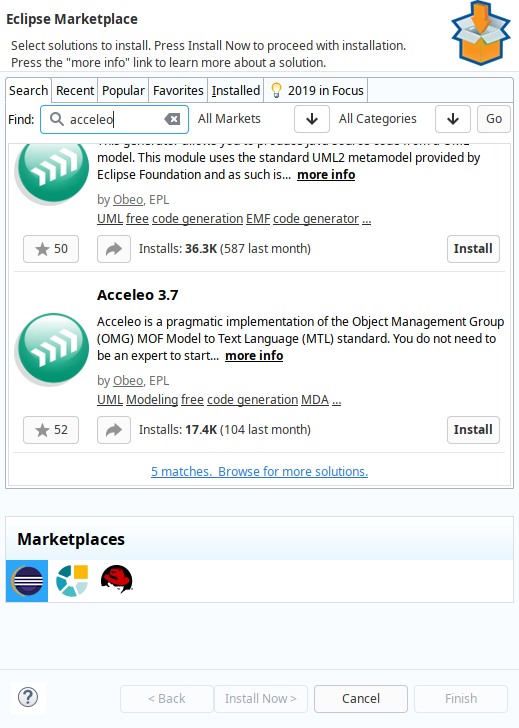
\includegraphics[width=.9\linewidth]{images/acceleo.png}
\end{center}

Similar a la instalación de \texttt{Papyrus}, se debe continuar el proceso de
instalación, al fin del cual se debe reiniciar \texttt{Eclipse}.

\section{Instalación}
\label{sec:orgb6f475c}
La instalación de los plugins es muy sencilla.

En primer lugar se debe contar con todos los plugins:

\begin{itemize}
\item Plugin mdcms, que provee el perfil UML.
\item Plugin mdcms2puppet, que provee la transformación de modelo mdcms a
código puppet.
\item Plugin mdcms2puppet-ui, que agrega un elemento al menú de click
derecho sobre los archivos .uml.
\end{itemize}

A continuación la instalación consiste en los siguientes simples
pasos:

\begin{enumerate}
\item Encontrar el directorio de instalación de \texttt{Eclipse}.
\item Ubicar allí el directorio "dropins".
\item Copiar los .jar de los plugins a dicho directorio.
\item Iniciar \texttt{Eclipse}.
\end{enumerate}

Luego de iniciar \texttt{Eclipse} se puede comprobar que los plugins están
instalados navegando a "Help > About Eclipse IDE > Installation
Details" y en la pestaña "Plugins" de la ventana que aparece, buscar
el nombre de los plugins.

\begin{center}
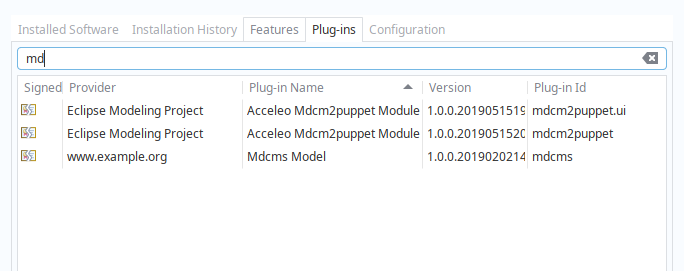
\includegraphics[width=.9\linewidth]{images/plugins.png}
\end{center}
\end{document}